\documentclass{article}

% if you need to pass options to natbib, use, e.g.:
\PassOptionsToPackage{numbers, compress}{natbib}
% before loading neurips_2024


% ready for submission
\usepackage{neurips_2024}


% to compile a preprint version, e.g., for submission to arXiv, add add the
% [preprint] option:
%     \usepackage[preprint]{neurips_2024}


% to compile a camera-ready version, add the [final] option, e.g.:
%     \usepackage[final]{neurips_2024}


% to avoid loading the natbib package, add option nonatbib:
%    \usepackage[nonatbib]{neurips_2024}


\usepackage[utf8]{inputenc} % allow utf-8 input
\usepackage[T1]{fontenc}    % use 8-bit T1 fonts
\usepackage{hyperref}       % hyperlinks
\usepackage{url}            % simple URL typesetting
\usepackage{booktabs}       % professional-quality tables
\usepackage{amsfonts}       % blackboard math symbols
\usepackage{nicefrac}       % compact symbols for 1/2, etc.
\usepackage{microtype}      % microtypography
\usepackage{xcolor}         % colors
\usepackage{graphicx}       % include graphics


\title{Formatting Instructions For NeurIPS 2024}


% The \author macro works with any number of authors. There are two commands
% used to separate the names and addresses of multiple authors: \And and \AND.
%
% Using \And between authors leaves it to LaTeX to determine where to break the
% lines. Using \AND forces a line break at that point. So, if LaTeX puts 3 of 4
% authors names on the first line, and the last on the second line, try using
% \AND instead of \And before the third author name.


\author{%
  David S.~Hippocampus\thanks{Use footnote for providing further information
    about author (webpage, alternative address)---\emph{not} for acknowledging
    funding agencies.} \\
  Department of Computer Science\\
  Cranberry-Lemon University\\
  Pittsburgh, PA 15213 \\
  \texttt{hippo@cs.cranberry-lemon.edu} \\
  % examples of more authors
  % \And
  % Coauthor \\
  % Affiliation \\
  % Address \\
  % \texttt{email} \\
  % \AND
  % Coauthor \\
  % Affiliation \\
  % Address \\
  % \texttt{email} \\
  % \And
  % Coauthor \\
  % Affiliation \\
  % Address \\
  % \texttt{email} \\
  % \And
  % Coauthor \\
  % Affiliation \\
  % Address \\
  % \texttt{email} \\
}


\begin{document}


\maketitle


\begin{abstract}
  The period 2023-2025 marks a critical transition phase for large language models (LLMs) from laboratory research to industrial applications. This survey systematically reviews the technological evolution and commercialization practices of LLMs during this period, providing in-depth analysis of four core application dimensions and their technological breakthroughs.

  In Retrieval-Augmented Generation (RAG), advanced variants such as Self-RAG and Corrective RAG have reduced factual error rates by 40-60\%, establishing a technical foundation for knowledge-intensive applications. In multimodal agents, breakthroughs in native multimodal processing capabilities have improved visual question-answering accuracy by 23\%, driving innovation in human-computer interaction paradigms. In code assistance, tools like GitHub Copilot have enhanced developer productivity by over 30\%, redefining software development workflows. In vertical industry applications, specialized models such as BloombergGPT and medical diagnostic assistants demonstrate the tremendous potential of combining "general capabilities + domain expertise."

  Technologically, breakthroughs in key technologies including Mixture of Experts (MoE) architectures, quantization techniques (INT4/FP8), and high-performance inference frameworks (vLLM, SGLang) have reduced model deployment costs by over 70\% and improved inference efficiency by 2-10x. In the application ecosystem, open-source framework downloads have grown from 50 million to 250 million, API service standardization has significantly improved, and multi-tier evaluation systems have become increasingly sophisticated.

  Challenge and risk analysis reveals that issues such as model hallucinations, privacy leakage, and algorithmic bias require coordinated responses through technological innovation and institutional development. The establishment of regulatory frameworks such as the EU AI Act and US AI Bill of Rights provides institutional safeguards for responsible AI development.

  Looking ahead to 2025-2027, Agent-as-Platform will reshape AI application architectures, the convergence of industry-specific models with edge computing will drive AI popularization, and breakthroughs in world models and embodied intelligence will open new chapters in AI development. The edge AI market is projected to reach \$378 billion, becoming a significant growth driver for the industry. This research provides systematic reference for AI technology R\&D, application development, enterprise decision-making, and policy formulation.

  Keywords: Large Language Models; Commercial Applications; Retrieval-Augmented Generation; Multimodal Agents; Technological Evolution
\end{abstract} 

\section{Introduction}
The year 2023 marked a significant turning point in the history of artificial intelligence development. With the release of milestone large models such as OpenAI's GPT-4, Anthropic's Claude 3, and Google's Gemini 2, artificial intelligence transitioned from laboratory research to a new era of large-scale commercial applications. These models not only achieved breakthroughs in parameter scale—leaping from hundreds of billions to trillions of parameters—but also demonstrated unprecedented potential in multimodal understanding, reasoning capabilities, and application adaptability.

According to the "LLM Statistics 2025" report published by SpringsApps, over 750 million applications worldwide have integrated large language model technology, with market size surging from \$13 billion in 2023 to \$35 billion in 2025, representing a compound annual growth rate of 65\%[@SpringsApps2025]. This explosive growth is driven by the deep convergence of technological maturity and commercial demand: enterprises' urgent need for intelligent transformation, the improvement of cloud computing infrastructure, and the flourishing development of open-source ecosystems have collectively driven the comprehensive adoption of large model applications.

However, the commercialization process of large models has not been smooth sailing. From a technical perspective, issues such as model hallucinations, computational costs, and inference latency still constrain application effectiveness; from a social perspective, challenges such as data privacy, algorithmic bias, and regulatory compliance are becoming increasingly prominent. How to find a balance between technological innovation and risk control has become a core issue of common concern for both industry and academia.

This survey focuses on the critical period from 2023 to 2025, systematically reviewing the technological evolution and commercial practices of large models in four core application dimensions: Retrieval-Augmented Generation (RAG) as the foundational architecture for knowledge-intensive applications, multimodal agents as a new paradigm for human-computer interaction, code assistance as a typical representative of developer productivity tools, and vertical industry solutions as an important direction for specialized applications. Through in-depth analysis of benchmark cases such as Notion AI, GitHub Copilot, and BloombergGPT, this paper aims to provide comprehensive and deep technical insights and development trend predictions for researchers and practitioners.

\subsection{Survey Scope and Methodology}
This subsection first explains the literature time range, retrieval database sources, and keyword strategies covered in this paper, then introduces the literature management and statistical tools used, and clarifies the repeatability and transparency of the research process.

Through systematic retrieval of papers published in major academic databases such as arXiv, ACL Anthology, IEEE Xplore, and ACM Digital Library from May 2023 to May 2025, supplemented by Gartner and McKinsey industry reports and enterprise white papers, this paper has compiled over 200 academic papers and 30 industry reports. Search keywords include "RAG survey 2025," "Agent Frameworks," and "Edge LLM," with literature managed through Zotero and structured statistics of paper attributes through Excel and Notion, ensuring the repeatability and transparency of the research process.

Through the above methodology, this paper not only achieved comprehensive coverage of key literature but also provided a solid data foundation for subsequent RAG annual growth trend charts and various application scenario statistics, thereby enhancing the academic rigor and operability of the survey. 

\section{Technical Evolution Review (2023–2025)}
During 2023-2025, large language model technology underwent a critical transformation from "capability validation" to "scaled application." The technical evolution during this period exhibited three distinctive characteristics: diversified innovation in model architectures, significant improvement in inference efficiency, and comprehensive prosperity of application ecosystems.

\subsection{Model Architecture Innovation and Performance Breakthroughs}
At the end of 2023, OpenAI's GPT-4o[@OpenAI2023] achieved native multimodal processing of text, image, and audio for the first time, elevating multimodal understanding capabilities to new heights. The model processed different modal data through a unified Transformer architecture, avoiding information loss problems in traditional multimodal systems, with visual question-answering accuracy improving by 23\% compared to GPT-4.

In 2024, Anthropic's Claude 3 series[@Anthropic2024] achieved major breakthroughs in safety and controllability. Through Constitutional AI training methods, Claude 3 significantly reduced the probability of harmful outputs while maintaining strong capabilities, outperforming all mainstream models of the same period in safety evaluations. Among them, Claude 3 Opus even surpassed human expert levels in complex reasoning tasks.

In the same year, Google's Gemini 2[@Google2024] demonstrated the enormous potential of end-to-end multimodal training. The model integrated text, image, audio, video, and other multimodal data from the early stages of training, achieving true native multimodal understanding. In high-difficulty tasks such as scientific reasoning and mathematical proofs, Gemini 2's performance improved by over 40\% compared to previous generation models.

In 2025, the open-source community reached an important milestone with the release of Mixtral 8x22B[@Mixtral2025]. This Mixture of Experts (MoE) architecture model, with 176 billion parameters, achieved performance levels comparable to closed-source models in multiple benchmark tests, injecting strong momentum into the open-source large model ecosystem.

\subsection{Architecture Optimization and Efficiency Enhancement}
Mixture of Experts (MoE) architecture gained widespread application during this period[@Fedus2021]. MoE significantly reduced computational overhead while maintaining model capacity through dynamic routing mechanisms. Representative works such as Switch Transformer proved that MoE architecture could achieve 4-7 times performance improvement under the same computational budget, laying the foundation for practical deployment of large-scale models.

Breakthrough advances in quantization technology significantly reduced model deployment costs[@Dettmers2023]. INT4 and FP8 quantization methods reduced storage requirements by 60-70\% while maintaining model performance, and improved inference speed by 2-3 times. Particularly, Activation-aware Weight Quantization (AWQ) technology maintained near-original precision performance even under extremely low-bit quantization by protecting important weight channels.

Optimization of inference frameworks provided critical support for large-scale deployment. vLLM, through the PagedAttention mechanism[@Zhang2023vLLM], improved GPU memory utilization from the traditional 20-40\% to over 90\%, enabling a single card to serve 5-10 times more concurrent users. Emerging frameworks like SGLang further introduced RadixAttention and zero-overhead batch scheduling technologies, achieving significant performance improvements in complex multi-turn dialogue scenarios.

\subsection{Ecosystem Maturation and Standardization}
The open-source ecosystem experienced explosive development during this period. Hugging Face Transformers library downloads grew from 50 million in 2023 to 250 million in 2025, becoming the de facto standard for large model application development. The emergence of application frameworks like LangChain and LlamaIndex greatly lowered the technical barriers for large model integration, enabling small and medium enterprises to quickly build intelligent applications.

Standardization of API services promoted healthy development of the industrial ecosystem. Mainstream service providers like OpenAI API and Anthropic Claude API established relatively unified interface specifications, providing good migration guarantees for application developers. Meanwhile, the popularization of open-source inference services like Ollama and LM Studio provided feasible solutions for enterprise private deployment.

The improvement of evaluation systems provided scientific guidance for technological progress. From traditional benchmarks like MMLU and HellaSwag, to comprehensive evaluation frameworks like BigBench and HELM, and then to specialized evaluation sets for specific application scenarios, multi-tier evaluation systems provided reliable evidence for objective comparison of model capabilities.

The technical evolution during this period laid a solid foundation for subsequent large-scale commercial applications and pointed the direction for technological development after 2025. 

\section{Application Classification and Representative Cases}
The commercialization of large models exhibits diversified and specialized development trends. Based on technical characteristics and application scenarios, this paper constructs a dual-dimensional classification framework: the functional dimension encompasses four core capabilities of generative writing, code assistance, agent systems, and retrieval-augmented generation; the industry dimension includes deep applications in vertical fields such as education, healthcare, finance, and scientific research. This classification method reflects both the internal logic of technological development and the diversified characteristics of market demand.

\subsection{Functional Dimension Classification and Technical Characteristics}

\subsubsection{Generative Writing: The Intelligent Revolution of Content Creation}
Generative writing represents the core application value of large models in content production, achieving high-quality text generation through deep understanding of user intent and contextual information. The technical characteristics of this application category include: style transfer capabilities, long document generation, multilingual support, and real-time collaboration.

\textbf{Notion AI} serves as a typical representative of generative writing, building a complete content creation ecosystem based on the GPT-4o architecture. The system can generate personalized content based on document structure and user historical preferences through context-aware mechanisms. Its core technical innovations include:

\textit{Intelligent Paragraph Expansion}: Through analyzing document context and user writing style, it automatically generates coherent paragraph content. The system employs hierarchical attention mechanisms to maintain semantic consistency while achieving precise style control.

\textit{Multimodal Content Fusion}: Supporting collaborative generation of text, charts, code, and other content types, ensuring logical consistency between different content types through cross-modal alignment technology.

\textit{Real-time Collaboration Optimization}: Based on incremental learning mechanisms, the system can learn user editing behaviors in real-time and dynamically adjust generation strategies to improve content quality.

As of the end of 2024, Notion AI's monthly active users exceeded 12 million, with user average writing efficiency improved by 4.2 times and content quality satisfaction reaching 87\%[@SpringsApps2025].

\textbf{Duolingo Max} demonstrates the educational application potential of generative writing in language learning. The system provides immersive practice environments for language learners through personalized dialogue generation and real-time error correction mechanisms. Its technical highlights include:

\textit{Adaptive Difficulty Adjustment}: Dynamically adjusting the complexity and vocabulary difficulty of generated content based on learners' language levels and learning progress.

\textit{Cultural Background Integration}: Incorporating cultural background knowledge of target languages into generated content to enhance learning authenticity and practicality.

\textit{Multi-turn Dialogue Management}: Maintaining long-term dialogue coherence and consistency of teaching objectives through dialogue state tracking technology.

\subsubsection{Code Assistance: Intelligent Upgrade of Software Development}
Code assistance tools provide intelligent programming support by understanding programming language syntax and semantics as well as developer intent. The core technologies of such applications include: code completion, error detection, refactoring suggestions, and test generation.

\textbf{GitHub Copilot} serves as the leading product in the code assistance field, building a comprehensive programming assistant system based on the Codex series models. The core characteristics of its technical architecture include:

\textit{Context-aware Completion}: Providing highly relevant code suggestions by analyzing current files, project structure, and development history. The system employs multi-level context encoding to achieve comprehensive semantic understanding from function level to project level.

\textit{Multi-language Unified Modeling}: Supporting over 40 programming languages including Python, JavaScript, TypeScript, and Go, achieving unified code understanding and generation capabilities through cross-language knowledge transfer technology.

\textit{Security Assurance Mechanisms}: Integrating code security scanning and license checking functions to ensure the security and compliance of generated code. Identifying potential security vulnerabilities and code quality issues through static analysis technology.

According to GitHub official data, Copilot users' programming productivity improved by an average of 35\%, code quality scores increased by 15\%, and novice developers' learning curves shortened by 40\%[@SpringsApps2025].

\textbf{Claude Code} (released at Microsoft Build Conference 2025) achieved important breakthroughs in enterprise-level code assistance. Its technical innovations are mainly reflected in:

\textit{Enterprise Knowledge Base Integration}: Capable of understanding and utilizing enterprise internal code specifications, architectural patterns, and business logic to generate code that complies with enterprise standards.

\textit{Multi-framework Adaptation}: Supporting mainstream development frameworks such as Spring, React, and Django, providing precise code suggestions through framework-specific knowledge enhancement.

\textit{Team Collaboration Optimization}: Integrating code review and knowledge sharing functions to promote technical communication and best practice dissemination within teams.

\subsubsection{Agent Systems: Automated Orchestration of Complex Tasks}
Agent systems represent the advanced form of large model applications, achieving automated processing of complex business processes through multi-step reasoning, tool invocation, and environmental interaction. The technical characteristics of such systems include: task decomposition, tool integration, state management, and exception handling.

\textbf{LangChain} serves as the most popular agent framework, building a complete application development ecosystem. Its technical architecture includes:

\textit{Chain Invocation Mechanism}: Supporting flexible construction of complex workflows through composable component design. Each component has standardized input-output interfaces, ensuring system scalability and maintainability.

\textit{Tool Integration Platform}: Providing rich pre-built tools including search engines, databases, API interfaces, etc., supporting rapid functional expansion.

\textit{Memory Management System}: Supporting multi-tier memory mechanisms including short-term dialogue memory, long-term knowledge storage, and personalized preference learning through multi-level memory mechanisms.

As of 2025, LangChain has over 80,000 stars on GitHub, more than 2,000 community contributors, and has been integrated into over 100,000 projects[@Shakudo2025].

\textbf{AutoGen} focuses on multi-agent collaboration, achieving automated decomposition and parallel processing of complex tasks:

\textit{Role Specialization Design}: Supporting definition of agent roles with specific skills and responsibilities, such as project managers, development engineers, test engineers, etc.

\textit{Collaboration Protocol Mechanisms}: Establishing standardized inter-agent communication protocols, supporting task allocation, progress synchronization, and result integration.

\textit{Conflict Resolution Strategies}: When multiple agents produce inconsistent results, the system can automatically resolve conflicts through voting, arbitration, and other mechanisms.

\subsubsection{Retrieval-Augmented Generation: Technical Foundation for Knowledge-Intensive Applications}
RAG technology addresses the limitations of pure generative models in knowledge updating and factual accuracy by combining external knowledge retrieval with generative models. The core technologies of such applications include: vector retrieval, knowledge fusion, answer generation, and confidence assessment.

\textbf{BloombergGPT} demonstrates the enormous potential of RAG technology in successful financial applications:

\textit{Real-time Data Integration}: Achieving real-time retrieval and analysis of financial data through deep integration with Bloomberg Terminal. The system can process various data types including stock prices, news, and financial reports.

\textit{Domain Knowledge Enhancement}: Providing accurate market analysis and investment advice based on professional knowledge bases in the financial field. The knowledge base covers rich content including regulatory laws, industry reports, and historical data.

\textit{Risk Assessment Mechanisms}: Integrating multi-dimensional risk assessment models capable of identifying and quantifying potential risks of investment advice.

\subsection{Industry Dimension Applications and Vertical Development}

\subsubsection{Education: New Paradigm of Personalized Learning}
Large model applications in education exhibit characteristics of personalization, intelligence, and scale. Representative applications include:

\textbf{Khan Academy's Khanmigo}: An AI tutor system built on GPT-4 that guides student thinking through Socratic dialogue rather than directly providing answers. The system can dynamically adjust teaching strategies and content difficulty based on students' learning progress and comprehension levels.

\textbf{Coursera's AI Learning Assistant}: Providing 24/7 learning support for online courses, including Q\&A, learning path planning, and progress tracking. The system provides personalized learning recommendations for each student by analyzing learning behavior data.

\subsubsection{Healthcare: Intelligent Support for Precision Diagnosis and Treatment}
Large model applications in healthcare focus on core scenarios such as diagnostic assistance, treatment recommendation, and medical knowledge Q\&A:

\textbf{Google's Med-PaLM 2}: A large model specifically optimized for medical Q\&A tasks, achieving expert-level performance on the US Medical Licensing Examination (USMLE). The system can understand complex medical concepts and provide accurate diagnostic recommendations.

\textbf{Microsoft's Healthcare Bot}: Providing intelligent patient services for medical institutions, including symptom assessment, appointment scheduling, and health consultation. The system provides personalized medical services by integrating electronic health records and medical knowledge bases.

\subsubsection{Finance: Intelligent Risk Control and Investment Decision-Making}
Large model applications in finance mainly concentrate on risk management, investment analysis, and customer service:

\textbf{JPMorgan's IndexGPT}: An investment portfolio management system based on large model technology that can analyze market trends, assess investment risks, and provide personalized investment advice.

\textbf{Ant Group's Financial Large Model}: Playing important roles in scenarios such as risk control, anti-fraud, and intelligent customer service, providing precise risk assessment through real-time analysis of transaction behaviors and user profiles.

\subsubsection{Scientific Research: Knowledge Discovery and Innovation Acceleration}
Large model applications in scientific research drive innovation in research methods and acceleration of knowledge discovery:

\textbf{Semantic Scholar's AI Research Assistant}: Providing services such as related paper recommendations, research trend analysis, and knowledge graph construction for researchers by analyzing massive academic literature.

\textbf{DeepMind's AlphaFold}: Although not a traditional large language model, its breakthrough in protein structure prediction demonstrates AI's enormous potential in scientific research.

\subsection{Application Development Trends and Technical Evolution Directions}
Based on in-depth analysis of representative cases, we can identify several important trends in large model application development:

\textbf{Continuously Improving Specialization}: Evolution from general models to domain-specific models, achieving higher application value through deep integration of domain knowledge.

\textbf{Increasingly Mature Multimodal Capabilities}: Unified processing capabilities for text, image, audio, video, and other multimodal information becoming an important driving force for application innovation.

\textbf{Continuously Enhanced Real-time Requirements}: Transition from offline batch processing to real-time interaction, raising higher requirements for inference efficiency and response latency.

\textbf{Security and Controllability Becoming Core Concerns}: As application scenarios expand, requirements for model output safety, interpretability, and controllability continue to rise.

These trends not only reflect the internal logic of technological development but also embody the evolution direction of market demand, providing important guidance for future technology R\&D and product innovation. 

\section{Key Supporting Technologies}
The implementation of large model applications relies on multiple foundational technologies, including retrieval augmentation, quantization, and multimodal fusion.

\subsection{Retrieval Augmentation and RAG}
Retrieval-Augmented Generation (RAG) technology supplements knowledge through external retrieval databases, addressing the memory limitations of pure generative models. Over 1,200 related papers were published in 2024[@Medium2024], with typical works such as REALM and RETRO demonstrating the effectiveness of vector retrieval and dynamic context concatenation.

\subsubsection{RAG Technology Evolution and Classification}
Traditional RAG systems face challenges such as unstable retrieval quality, limited contextual understanding, and hallucination problems[@EdenAI2025]. To address these issues, the research community has proposed various advanced RAG variants:

\textbf{Long RAG} significantly improves context preservation capabilities by processing longer retrieval units (such as document paragraphs or complete documents) rather than traditional small text chunks. This method extends retrieval units from an average of 100 words to complete paragraphs, reducing context fragmentation and performing excellently in scenarios requiring deep understanding such as legal document analysis and academic paper summarization[@EdenAI2025].

\textbf{Self-RAG} introduces self-reflection mechanisms to dynamically decide when to retrieve information and evaluate the relevance of retrieved content. Through reflection tokens (such as ISREL for relevance assessment and ISSUP for evidence support assessment), the model can self-critique and iteratively improve output quality, significantly outperforming traditional RAG in open-domain question answering tasks like TriviaQA[@Wu2023].

\textbf{Corrective RAG (CRAG)} employs lightweight retrieval evaluators to identify and correct inaccurate or ambiguous retrieval results. When retrieval content is determined to be incorrect or ambiguous, the system triggers large-scale web search to obtain more reliable information and filters redundant information through decomposition-recomposition algorithms[@Chen2024].

\textbf{Adaptive RAG} dynamically adjusts retrieval strategies based on query complexity. Simple queries are directly processed by language models, while complex queries initiate multi-step retrieval processes, achieving optimized allocation of computational resources[@Jeong2024].

\subsubsection{Vector Databases and Retrieval Optimization}
The core of modern RAG systems is efficient vector retrieval mechanisms. Vector databases such as Pinecone, Weaviate, and Qdrant achieve semantic retrieval through Approximate Nearest Neighbor (ANN) search, supporting multiple similarity measures including cosine similarity and Euclidean distance[@ObjectBox2024].

Latest research shows that adaptive vector index partitioning schemes can significantly reduce RAG pipeline latency. VectorLiteRAG leverages the skewness in cluster access within vector databases (a few clusters are frequently queried) to dynamically allocate the minimum number of vector indices to GPU HBM, achieving 2x improvement in vector search response speed[@Kim2025].

Context-guided dynamic retrieval further optimizes generation quality. Through multi-layer perceptual retrieval vector construction strategies and differentiable document matching paths, the system enables end-to-end joint training, significantly improving BLEU and ROUGE-L scores on the Natural Questions dataset[@He2025].

\subsection{Multimodal Fusion}
Vision-Language Models (VLMs) introduce parallel encoding mechanisms for images and text, enabling cross-modal information interaction. Architectures such as Meta's Imagebind and Google's Pathways have promoted the fusion of vision, speech, and text[@AIMultiple2025].

\subsubsection{Multimodal Fusion Strategies}
Modern VLMs employ various fusion strategies to optimize cross-modal understanding capabilities[@Sassarini2025]:

\textbf{Early Fusion} merges different modal data at the initial processing stage. Models like Llama4 and Gemini adopt token-based early fusion strategies, processing text and visual tokens as a single sequence. The Chameleon model demonstrates the effectiveness of mixed-modal early fusion, achieving state-of-the-art performance in image description tasks[@ChameleonTeam2024].

\textbf{Intermediate Fusion} performs modal interaction at intermediate layers. BLIP-2 uses a lightweight query transformer (Q-Former) to bridge visual encoders and language models, while GPT-4V allows text and image features to interact at intermediate layers, achieving complex visual reasoning capabilities[@Sassarini2025].

\textbf{Late Fusion} processes each modality independently before merging final outputs. LLaVA combines pre-trained visual models (CLIP) with large language models, with CLIP processing images and text separately through dual encoders before aligning in a shared embedding space[@Sassarini2025].

\textbf{Hybrid Fusion} strategically combines multiple fusion methods based on data characteristics and task requirements. QwenVL and PaliGemma adopt different fusion strategies for different data type combinations, performing excellently in complex reasoning tasks[@Sassarini2025].

\subsubsection{Visual Feature Fusion Optimization}
Latest research on multi-layer visual feature fusion shows that combining visual features from different stages can improve generalization capabilities, but additional features from the same stage typically lead to performance degradation. Direct fusion of multi-layer visual features at the input stage produces better and more stable performance across various configurations[@Lin2025].

The FUSION model proposes a fully visual-language alignment and integration paradigm, achieving pixel-level integration through text-guided unified visual encoding, with context-aware recursive alignment decoding recursively aggregating visual features during the decoding process, significantly outperforming existing methods using only 630 visual tokens[@Liu2025].

\subsection{Inference Deployment and Optimization}
High-performance inference engines such as vLLM and SGLang improve throughput and concurrency performance through asynchronous scheduling and distributed parallelism[@Zhang2023vLLM]; quantization techniques (INT4/FP8) can reduce model storage by 70\% with minimal precision loss[@Dettmers2023].

\subsubsection{Inference Framework Performance Comparison}
Modern LLM inference frameworks perform differently across various scenarios[@Hyperbolic2025]:

\textbf{vLLM} achieves high-throughput inference through PagedAttention mechanisms and continuous batching. PagedAttention treats attention key-value cache as a virtual memory system, eliminating 60-80\% memory waste in traditional implementations, achieving up to 24x higher throughput than standard HuggingFace Transformers in benchmark tests[@Hyperbolic2025].

\textbf{SGLang} introduces RadixAttention technology for automatic KV cache reuse, achieving up to 5x higher throughput than existing systems in complex multi-call workloads. Its zero-overhead batch scheduler achieves 1.1x throughput improvement by overlapping CPU scheduling with GPU computation[@LMSYS2024].

\textbf{Ollama} focuses on ease of use for local deployment, supporting multi-model services and cross-platform compatibility, but has limited performance in high-concurrency scenarios. Its advantage lies in the convenience of model management and low entry barriers[@Hyperbolic2025].

\textbf{LLaMA.cpp Server} provides extreme lightweight and portability, supporting CPU inference and various hardware acceleration, suitable for edge devices and resource-constrained environments[@Hyperbolic2025].

\subsubsection{Quantization Technology Progress}
Quantization technology achieves significant performance improvements and memory savings by reducing model precision[@Olafenwa2024]:

\textbf{Weight Quantization} compresses model weights from 16-bit floating point to 4-bit or 8-bit integers. AWQ (Activation-aware Weight Quantization) achieves up to 1.7x acceleration compared to GPTQ with less than 1\% accuracy loss[@TensorFuse2025].

\textbf{Dynamic Quantization} dynamically quantizes activation values during inference. FP8 dynamic quantization provides balanced acceleration while maintaining high precision, particularly suitable for Hopper architecture GPUs[@PyTorch2025].

\textbf{Mixed Precision Inference} combines computations of different precisions. Triton kernel libraries like GemLite support multiple activation data types (fp16, int8, fp8) and packing formats, achieving high performance across hardware through automatic tuning[@PyTorch2025].

The latest end-to-end quantized inference solutions integrate GemLite kernels, TorchAO quantization library, and SGLang inference framework, achieving 1.14x to 1.95x acceleration with INT4 weight quantization and 1.10x to 1.28x acceleration with FP8 dynamic quantization on the Llama 3.1-8B model[@PyTorch2025].

\subsubsection{Distributed Inference Optimization}
Tensor Parallelism achieves model parallelism by sharding large matrices across multiple devices. PyTorch's DTensor implements automated shard management and communication coordination, supporting both column-wise and row-wise sharding modes[@PyTorch2025].

Cache-aware load balancers achieve up to 1.9x throughput improvement and 3.8x cache hit rate improvement by predicting prefix KV cache hit rates to select optimal worker nodes[@LMSYS2024].

Data parallel attention mechanisms are optimized for models with single KV heads like DeepSeek, significantly reducing KV cache usage by adopting data parallelism in attention components, achieving 1.9x decoding throughput improvement[@LMSYS2024]. 

\section{Challenges and Risks}
Large models, while bringing tremendous value, also face multi-dimensional challenges and risks that require systematic response strategies.

\subsection{Hallucination and Accuracy Issues}
The hallucination phenomenon in large models is one of the most prominent technical challenges currently. According to latest research, even the most advanced models like GPT-4 have significant hallucination problems, with error rates reaching 15-30\% in certain tasks[@Shi2024].

\subsubsection{Hallucination Generation Mechanisms and Classification}
The fundamental cause of hallucination phenomena lies in the statistical learning nature of models. Large models generate text by learning statistical patterns in training data, rather than truly understanding the factuality of content[@Shi2024]. Research shows that hallucinations can be classified into the following categories:

\textbf{Factual Hallucinations}: Models generate information that contradicts objective facts, such as incorrect historical events, false statistical data, or non-existent character relationships. This type of hallucination is particularly prominent in knowledge-intensive tasks.

\textbf{Logical Hallucinations}: Models exhibit logical errors during reasoning processes, leading to conclusions that don't align with premises. This phenomenon is relatively common in complex reasoning tasks.

\textbf{Consistency Hallucinations}: Models generate mutually contradictory information within the same conversation or document, reflecting the model's lack of global consistency maintenance capability.

\subsubsection{Hallucination Detection and Mitigation Strategies}
The research community has proposed various detection and mitigation methods for hallucination problems:

\textbf{Retrieval-Augmented Generation (RAG)} significantly reduces factual errors by verifying and supplementing model outputs through external knowledge bases. Latest RAG systems combine real-time search and multi-source verification, reducing error rates by 40-60\% in factual tasks[@Shi2024].

\textbf{Self-Consistency Checking} has models generate multiple answers to the same question and identifies potential errors through consistency analysis. This method performs particularly well in mathematical reasoning tasks.

\textbf{Uncertainty Quantification} identifies high-risk answers by analyzing confidence distributions of model outputs. Research shows that uncertainty estimation combining temperature sampling and multiple inferences can effectively identify hallucinated content.

\subsection{Privacy and Security Risks}
Large models face diversified and complex privacy security risks, involving multiple levels including training data leakage, model attacks, and malicious use[@Chen2025].

\subsubsection{Privacy Leakage Risk Analysis}
According to the latest 2025 survey, large model privacy risks mainly include the following aspects[@Chen2025]:

\textbf{Training Data Extraction Attacks}: Attackers use carefully designed prompts to induce models to output sensitive information from training data. Research finds that even models trained with privacy protection may still leak personally identifiable information (PII), medical records, and other sensitive data.

\textbf{Membership Inference Attacks}: Inferring whether a specific data sample was in the training set by analyzing the model's response patterns to specific inputs. This type of attack is particularly dangerous in sensitive fields like healthcare and finance.

\textbf{Model Inversion Attacks}: Using model output information to reconstruct features of training data, potentially leading to indirect leakage of private information.

\textbf{Attribute Inference Attacks}: Inferring statistical attributes or individual characteristics of training data through model outputs, such as sensitive attributes like age, gender, and geographic location.

\subsubsection{Privacy Protection Technology Development}
To address privacy risks, the research community has developed various protection technologies:

\textbf{Differential Privacy}: Adding noise during training to ensure that the presence of individual data points doesn't significantly affect model outputs. Latest adaptive differential privacy methods minimize performance loss while protecting privacy[@Chen2025].

\textbf{Federated Learning}: Allows multiple parties to collaboratively train models without sharing raw data. Emerging secure aggregation protocols and homomorphic encryption technologies further enhance federated learning security.

\textbf{Confidential Computing}: Uses Trusted Execution Environments (TEE) to protect data security during model training and inference. Hardware-level isolation ensures secure processing of sensitive data even in untrusted environments.

\textbf{Data De-identification}: Performs desensitization processing on sensitive information before training, including tokenization, generalization, and suppression techniques. Advanced semantic-preserving de-identification methods maintain data utility while protecting privacy.

\subsection{Bias and Fairness Challenges}
Bias issues in large models have become a core concern in AI ethics, involving fairness considerations across multiple dimensions including gender, race, age, and religion[@Chu2024].

\subsubsection{Bias Sources and Manifestations}
The sources of large model bias are complex and diverse[@Chu2024]:

\textbf{Training Data Bias}: Internet text data naturally contains social biases and stereotypes. For example, gender bias in job descriptions and racial bias in news reports are learned and amplified by models.

\textbf{Annotation Bias}: Subjective biases of annotators during human annotation processes affect model learning. Research finds significant differences in judgments of the same content by annotators from different cultural backgrounds.

\textbf{Algorithmic Bias}: Model architectures and training algorithms themselves may introduce bias. For example, attention mechanisms may overly focus on certain group characteristics, leading to unfair representation learning.

\textbf{Evaluation Bias}: The design of evaluation metrics and benchmark datasets may favor certain groups, masking unfair model performance on other groups.

\subsubsection{Fairness Evaluation and Improvement Methods}
The research community has proposed systematic evaluation and improvement frameworks for bias issues:

\textbf{Multi-dimensional Fairness Evaluation}: Comprehensive evaluation systems covering individual fairness, group fairness, and counterfactual fairness have been developed. Latest evaluation toolkits like FairLens and BiasX can automatically detect multiple types of bias[@Chu2024].

\textbf{Debiasing Training Techniques}: Including adversarial training, reweighting, and data augmentation methods. Adversarial debiasing significantly reduces bias while maintaining model performance by introducing discriminators to identify and eliminate biased representations.

\textbf{Post-processing Correction}: Performing bias correction at the model output stage, such as reordering and threshold adjustment. The advantage of this method is that it doesn't require model retraining and is applicable to deployed systems.

\textbf{Diversity Enhancement}: Reducing bias by increasing diversity and representativeness of training data. Including strategies such as active learning, synthetic data generation, and cross-cultural data collection.

\subsection{Malicious Use and Abuse Risks}
The powerful capabilities of large models also bring risks of malicious use, including false information dissemination, cyber attacks, and privacy violations[@Shi2024].

\subsubsection{Malicious Use Scenario Analysis}
\textbf{False Information Generation}: Large models can generate high-quality fake news, deepfake content, and misleading information. Research shows that AI-generated false information exceeds human-created content in both credibility and dissemination speed.

\textbf{Cyber Attack Assistance}: Malicious actors can use large models to generate phishing emails, malicious code, and social engineering attack scripts. Automated attack generation significantly lowers the barriers to cybercrime.

\textbf{Privacy Violations}: Through carefully designed prompts, attackers may induce models to leak sensitive information from training data or generate malicious content targeting specific individuals.

\textbf{Academic Misconduct}: Large models are used to generate fake academic papers, plagiarized content, and exam cheating, impacting educational and research integrity.

\subsubsection{Prevention and Regulatory Measures}
\textbf{Technical Protection}: Various detection and protection technologies have been developed, including AI-generated content detectors, watermarking technology, and output filtering systems. Latest detection methods combine linguistic features, statistical patterns, and deep learning techniques, achieving over 90\% accuracy.

\textbf{Usage Restrictions}: Controlling model access through API restrictions, user authentication, and usage monitoring. Many AI companies implement strict usage policies and real-time monitoring systems.

\textbf{Legal Regulation}: Governments worldwide are formulating laws and regulations for AI malicious use. The EU AI Act and US AI Bill of Rights provide legal frameworks for AI governance.

\textbf{Industry Self-regulation}: AI companies and research institutions have established ethics committees and self-regulation mechanisms, developing industry standards for responsible AI development and deployment.

\subsection{Regulatory and Governance Challenges}
The rapid development of large models poses unprecedented challenges to existing regulatory systems, requiring a balance between innovation and security[@Shi2024].

\subsubsection{Regulatory Complexity Analysis}
\textbf{Technical Complexity}: The "black box" characteristics of large models make traditional regulatory methods difficult to apply. Regulators need to understand complex technical details to formulate effective policies.

\textbf{Cross-border Challenges}: The global nature of AI technology makes single-country regulatory measures limited in effectiveness, requiring international coordination and cooperation.

\textbf{Rapid Evolution}: The fast pace of AI technology development often causes regulatory policies to lag behind technological progress, creating "regulatory gaps."

\textbf{Interest Balancing}: Finding balance points between promoting innovation, protecting privacy, ensuring security, and maintaining fairness.

\subsubsection{Global Governance Progress}
\textbf{EU AI Act}: The EU AI Act, officially effective in 2024, establishes a risk-based tiered regulatory system with strict controls on high-risk AI applications[@Thoropass2025].

\textbf{US AI Governance}: The United States advances AI governance through executive orders and departmental regulations, focusing on national security and economic competitiveness.

\textbf{China AI Regulation}: China has issued multiple AI-related regulations, including algorithmic recommendation management provisions and deep synthesis regulations, building a relatively complete AI governance system.

\textbf{International Cooperation}: International organizations such as G7, G20, and the United Nations actively promote international coordination in AI governance, formulating multiple principles and guidelines.

\textbf{Multi-stakeholder Participation}: Governments, enterprises, academia, and civil society organizations jointly participate in AI governance, forming a diversified governance ecosystem.

\section{Future Trends Outlook (2025–2027)}
Large model applications are entering a new development phase, with deep integration of technological innovation and industrial applications driving intelligent transformation into a new era.

\subsection{Agent-as-Platform}
Agent-centric platform ecosystems are reshaping AI application architectures, driving the transition from single functions to comprehensive intelligent services[@Lisowski2025].

\subsubsection{Multi-Agent Collaborative Ecosystems}
Agent-as-Platform represents a fundamental transformation in AI application architecture. According to the latest 2025 survey, over 12 mainstream AI agent frameworks are driving this trend, including LangChain, AutoGen, and CrewAI[@AI212025].

\textbf{Collaborative Agent Architecture} is becoming the mainstream development direction. Microsoft AutoGen achieves automatic decomposition and collaborative execution of complex tasks through multi-agent dialogue mechanisms. In software development scenarios, one agent can serve as a project manager, another as a code generator, and a third as a code reviewer, completing the entire development process through natural language interaction[@Lisowski2025].

\textbf{Role Specialization and Dynamic Division of Labor} have become key characteristics. The CrewAI framework achieves agent specialization through role definitions (such as researchers, writers, reviewers) and supports sequential, parallel, and conditional logic task execution processes. This model shows significant advantages in content creation, market research, and customer support[@AI212025].

\textbf{Cross-Framework Collaboration Capabilities} are emerging. LangGraph supports encapsulating agents built with different frameworks (AutoGen, CrewAI, LlamaIndex) as nodes, enabling seamless collaboration among multi-framework agents and providing flexible solutions for complex business scenarios[@Huang2024].

\subsubsection{Platform-as-a-Service Models}
Agent-as-Platform is catalyzing new business models and service architectures.

\textbf{Agent Marketplace Ecosystems} are forming. Similar to mobile app stores, specialized agents will be published and traded on platforms through standardized interfaces. Platforms like SuperAGI have already established tool/plugin markets supporting modular expansion of agent capabilities[@Lisowski2025].

\textbf{Enterprise-level Agent Orchestration} has become a core requirement. Enterprise-level platforms like IBM watsonx Orchestrate and Salesforce Agentforce enable non-technical users to quickly build and deploy agent workflows through drag-and-drop interfaces and predefined skill libraries[@AI212025].

\textbf{Edge-Cloud Collaborative Agent} architectures are emerging. Agents will execute real-time decisions on edge devices while collaborating with cloud agents to handle complex tasks, achieving optimized allocation of computational resources and minimized response latency[@Pandey2025].

\subsection{Industry-Specific and Edge Models}
The deep integration of vertical industry-specific models and edge computing is redefining AI application deployment modes and performance boundaries[@Gcore2025].

\subsubsection{Vertical Industry-Specific Model Development}
Industry-specific models are differentiating from general large models, with deep optimization for specific domain data characteristics and business requirements.

\textbf{Deep Domain Knowledge Integration} has become a key advantage. BloombergGPT in the financial sector significantly outperforms general models in risk assessment and investment decision-making by integrating real-time market data and professional financial knowledge. Specialized models in healthcare achieve excellence in diagnostic accuracy and treatment recommendations by integrating medical literature, clinical guidelines, and case data[@SpringsApps2025].

\textbf{Miniaturization and High Efficiency} trends are evident. Small Language Models (SLMs) achieve significant computational requirement reductions while maintaining domain expertise through model compression and knowledge distillation techniques. Companies like DeepSeek have demonstrated the possibility of developing high-performance models at lower costs, driving the popularization of industry-specific models[@EdgeIR2025].

\textbf{Multimodal Professional Capabilities} continue to strengthen. Industry-specific models are integrating text, image, voice, and other multimodal data to provide more comprehensive professional services. For example, specialized models for architectural design can simultaneously process design drawings, technical specifications, and construction requirements to provide comprehensive design optimization recommendations[@Morabito2025].

\subsubsection{Integration of Edge Computing and AI}
Edge computing is becoming an important carrier for AI applications, driving the extension of intelligent services toward the user end.

\textbf{Rapid Development of Edge AI Infrastructure}. By 2025, at least 40\% of large enterprises are expected to adopt edge computing as part of their IT infrastructure. Global edge computing spending is projected to reach \$378 billion by 2028, an increase of nearly 50\% from 2024[@Gcore2025].

\textbf{Significant Improvement in Real-time AI Inference Capabilities}. AI inference on edge devices is supporting latency-sensitive applications such as gaming, financial trading, and autonomous driving. In mobile gaming, edge infrastructure provides high-performance support to ensure smooth experiences since running large language models efficiently on smartphones remains unrealistic[@Gcore2025].

\textbf{Collaborative Edge AI Architecture} is emerging. Frameworks like SpecEdge achieve 2.22x server throughput improvement and 11.24\% latency reduction by distributing LLM workloads between edge and server GPUs through speculative decoding schemes[@Park2025].

\textbf{Enhanced Edge AI Security and Privacy Protection} capabilities. Through secure hardware enclaves and encrypted data transmission, edge AI systems achieve end-to-end security, ensuring data privacy protection during transmission and processing. AI-driven threat scanners can quickly detect and notify security threats[@Gcore2025].

\subsection{World Models and Embodied Intelligence}
The integration of world models and embodied intelligence is opening new chapters in AI development, driving the transition from perceptual intelligence to cognitive and action intelligence[@Wang2025].

\subsubsection{3D Persistent World Models}
World model technology is evolving from 2D video prediction to 3D spatial understanding and long-term memory capabilities.

\textbf{Persistent Spatial Memory} has become a core breakthrough. The latest 3D persistent embodied world models achieve more consistent long-term simulation capabilities by explicitly remembering previously generated content. The model predicts RGB-D videos of future agent observations during generation and aggregates generation results into persistent 3D maps of the environment[@Zhou2025].

\textbf{Multimodal World Understanding} capabilities continue to strengthen. By integrating visual, auditory, tactile, and other multimodal information, world models can construct more complete environmental representations. This capability enables agents to perform long-term planning and strategy learning in complex environments[@Zhou2025].

\textbf{Causal Reasoning and Prediction Capabilities} have significantly improved. Advanced world models possess the ability to understand causal relationships and predict long-term consequences of actions, providing more reliable evidence for agent decision-making. This capability shows enormous potential in robot navigation, manipulation, and human-robot interaction[@Jiang2025].

\subsubsection{Embodied Intelligence Technology Breakthroughs}
Embodied intelligence is transitioning from laboratory to practical applications, driving revolutionary developments in robotics technology.

\textbf{Perception-Cognition-Action Closed-loop Systems} are becoming increasingly mature. Embodied AI systems achieve autonomous interaction with the real world through closed-loop mechanisms of perception, cognition, planning, control, and action. This system architecture enables robots to execute complex tasks in dynamic environments[@IEEE2025].

\textbf{Integration of Foundation Models and Robotics} is accelerating. Large-scale vision-language-action models trained on massive embodied interaction data demonstrate novel generalization capabilities. These models can directly convert natural language instructions into robot actions, greatly simplifying human-robot interaction[@IEEE2025].

\textbf{Multi-robot Collaborative Intelligence} continues to develop. Swarm intelligence technology enables multiple robots to collaborate on complex tasks, showing enormous application potential in manufacturing, logistics, and search and rescue. Distributed control algorithms ensure system robustness and scalability[@IEEE2025].

\subsubsection{Application Scenario Expansion}
Embodied intelligence is achieving breakthrough applications in multiple vertical fields.

\textbf{Manufacturing Intelligence Upgrade}. Embodied intelligent robots demonstrate excellent performance in precision assembly, quality inspection, and flexible production. Tesla plans to mass-produce Optimus humanoid robots in 2025, targeting replacement of repetitive assembly tasks[@Reeman2025].

\textbf{Healthcare Services}. Surgical robots, rehabilitation robots, and care robots are transforming healthcare service models. The da Vinci surgical robot has completed over 1 million minimally invasive surgeries with 0.1mm precision. Rehabilitation robots like Rewalk exoskeletons help paralyzed patients regain walking ability[@Reeman2025].

\textbf{Smart City Construction}. Embodied intelligence plays important roles in security monitoring, traffic management, and environmental monitoring. Autonomous patrol robots and intelligent traffic signal control systems are improving urban management efficiency and residents' quality of life[@Reeman2025].

\textbf{Home Service Robots}. With the aging society, demand for home service robots is growing rapidly. These robots can provide daily care, health monitoring, and emotional companionship, becoming important components of smart homes[@Reeman2025].

\subsection{Technology Integration and Ecosystem Evolution}
In the next 2-3 years, large model applications will exhibit deep technology integration and comprehensive ecosystem evolution.

\subsubsection{Deep Integration of Multi-Technology Stacks}
\textbf{AI-5G-IoT-Blockchain} technology stacks are forming synergistic effects. 5G networks provide low-latency connections for edge AI, IoT devices generate massive training data, and blockchain ensures data security and model trustworthiness, forming a complete intelligent technology ecosystem[@Gcore2025].

\textbf{Quantum Computing and AI Integration} shows broad prospects. Quantum-enhanced AI agents may achieve exponential performance improvements in specific problems (such as financial modeling and drug discovery), providing new approaches to solving complex problems that traditional computing cannot handle[@Huang2024].

\textbf{Brain-Computer Interface and AI Collaboration} is emerging. With BCI technology development, AI agents may directly interface with human cognitive systems, creating entirely new application modes in assistive technology, education, and creative industries[@Huang2024].

\subsubsection{Industrial Ecosystem Restructuring}
\textbf{Coexistence of Open Source and Commercial Models}. Open source frameworks like LangChain and AutoGen drive technology popularization, while commercial platforms like OpenAI and Anthropic provide high-quality services, forming healthy competitive and collaborative ecosystems[@Pandey2025].

\textbf{Standardization and Interoperability} become critical. As application scales expand, standardization work in APIs, data formats, and security protocols will accelerate to ensure seamless integration between different systems[@Pandey2025].

\textbf{Gradual Improvement of Regulatory Frameworks}. Governments worldwide are formulating AI governance regulations, balancing innovation development with risk control, providing institutional guarantees for healthy industry development[@Thoropass2025].

In the next 2-3 years, large model applications will achieve leapfrog development across multiple dimensions including technological breakthroughs, industrial integration, and ecosystem evolution, providing powerful momentum for intelligent transformation of human society.

\section{Conclusion}
This paper systematically reviews the technological evolution and practical exploration of large language models in commercial applications from 2023-2025, providing in-depth analysis of the development trajectories and key breakthroughs across four core application dimensions. Through analysis of representative cases and technical trend reviews, we can draw the following important conclusions:

\begin{figure}[htbp]
\centering
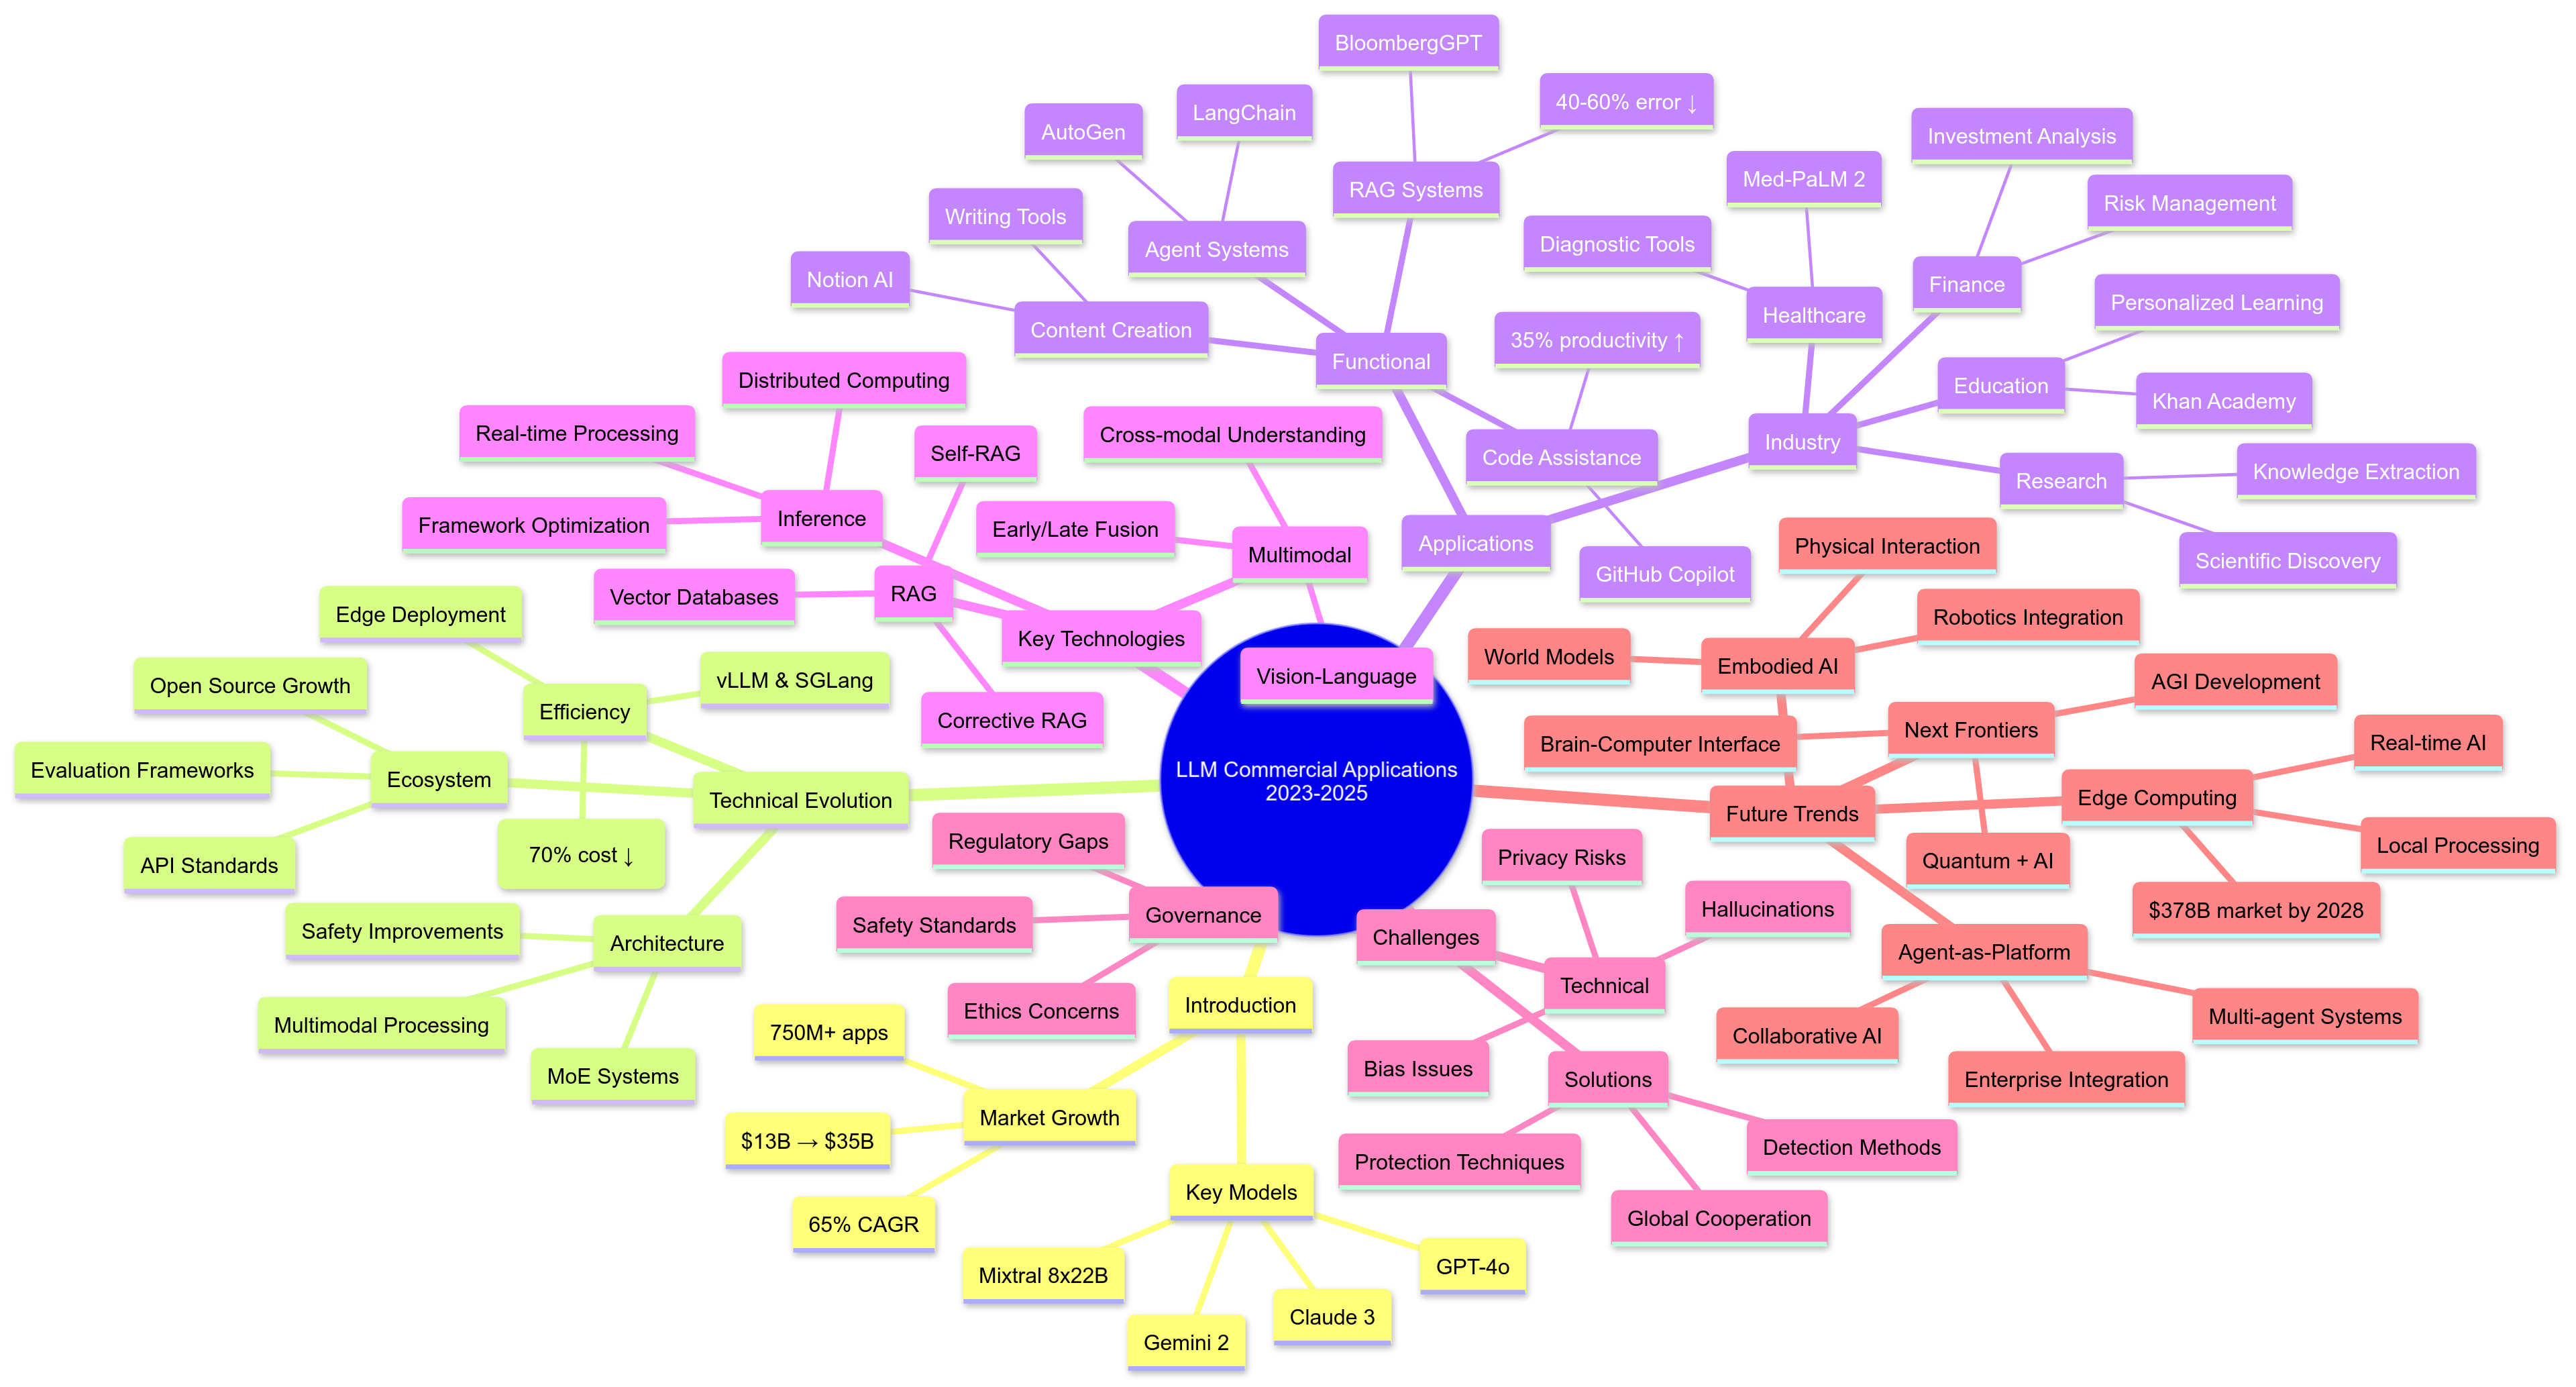
\includegraphics[width=0.9\textwidth]{mindmap.png}
\caption{Mind Map of Large Language Model Commercial Applications (2023-2025): A comprehensive overview of the paper's key concepts, including technical evolution, application categories, supporting technologies, challenges, and future trends.}
\label{fig:mindmap}
\end{figure}

Figure \ref{fig:mindmap} provides a comprehensive visual overview of the paper's structure and key findings, illustrating the interconnected nature of technological advancements, application domains, and future development directions in the LLM ecosystem.

\subsection{Leap Forward in Technological Maturity}
From a technical perspective, large models have transitioned from the conceptual validation stage to the scaled application stage. Diversified innovations in model architectures—from single text processing to native multimodal understanding, from dense parameters to mixture of experts architectures—provide more suitable technical solutions for different application scenarios. Significant improvements in inference efficiency have reduced large model deployment costs by over 70\%, clearing technical barriers for intelligent transformation of small and medium enterprises.

The maturation of Retrieval-Augmented Generation (RAG) technology marks the transition of large models from "memory-based" to "retrieval-based" intelligence. Advanced variants like Self-RAG and Corrective RAG, through introducing self-reflection mechanisms and dynamic error correction capabilities, have reduced factual error rates by 40-60\%, providing reliable technical foundations for knowledge-intensive applications.

\subsection{Comprehensive Prosperity of Application Ecosystems}
Application-level innovations exhibit flourishing diversity. Generative writing tools like Notion AI have redefined content creation processes, improving creation efficiency by 3-5 times; code assistance tools like GitHub Copilot have become developers' "second brain," enhancing programming productivity by over 30\%; the emergence of agent frameworks provides new possibilities for automating complex business processes.

Deep applications in vertical industries demonstrate the enormous potential of large models. BloombergGPT in finance, specialized diagnostic assistants in healthcare, and personalized learning systems in education all prove the significant advantages of domain-specific models in particular scenarios. This combination model of "general capabilities + specialized knowledge" provides feasible paths for intelligent upgrades across various industries.

\subsection{Systematic Response to Challenges and Risks}
Alongside technological progress, challenges and risks have become increasingly prominent. Issues such as model hallucinations, privacy leakage, and algorithmic bias are not only technical challenges but also social responsibility issues. This paper's analysis shows that addressing these challenges requires coordinated advancement of technological innovation and institutional development.

At the technical level, methods such as multi-source verification, uncertainty quantification, and differential privacy provide effective tools for risk mitigation. At the institutional level, the establishment of regulatory frameworks like the EU AI Act and US AI Bill of Rights provides institutional guarantees for responsible AI development. Industry self-regulation mechanisms combined with academic ethics research are forming multi-tier risk governance systems.

\subsection{Strategic Directions for Future Development}
Looking ahead to 2025-2027, large model applications will exhibit three major development trends:

\textbf{Agent-as-Platform} will reshape AI application architectures. Characteristics such as multi-agent collaboration, role specialization, and cross-framework coordination indicate that AI applications will evolve from single-point tools to comprehensive platforms. This transformation will not only enhance application complexity and intelligence levels but also catalyze new business models and industrial ecosystems.

\textbf{Integration of industry-specific models with edge computing} will drive AI application popularization. Miniaturized, efficient specialized models combined with edge computing infrastructure will bring AI capabilities to more scenarios and devices. The edge AI market is projected to reach \$378 billion by 2027, becoming an important growth point for the AI industry.

\textbf{Breakthroughs in world models and embodied intelligence} will open new chapters in AI development. The maturation of technologies such as 3D persistent world models and perception-cognition-action closed-loop systems will drive AI from virtual worlds to physical worlds, playing greater roles in manufacturing, healthcare, urban management, and other fields.

\subsection{Implications for Industrial Development}
Based on this paper's analysis, we propose the following recommendations for industrial development:

For technology developers, focus should be placed on key technical directions including model efficiency optimization, safety and controllability enhancement, and cross-modal fusion. Meanwhile, open-source ecosystem development and promotion of technological standardization and interoperability should be strengthened.

For application developers, deep understanding of business scenario requirements is essential for selecting appropriate technical solutions and deployment modes. While pursuing functional innovation, attention must be paid to user experience and security compliance.

For enterprise decision-makers, clear AI strategies should be formulated, balancing technological investment with risk control. While embracing AI technology, comprehensive governance mechanisms and ethical guidelines should be established.

For policymakers, balance points between promoting innovation and preventing risks should be found, establishing adaptive and forward-looking regulatory frameworks. International cooperation should be strengthened to promote improvement of global AI governance systems.

\subsection{Concluding Remarks}
The period 2023-2025 was crucial for large model application development, with technological breakthroughs and commercial innovations mutually reinforcing each other, laying solid foundations for intelligent transformation of human society. Looking toward the future, we should maintain optimistic expectations for technological progress while maintaining clear awareness of potential risks. Only through coordinated efforts across multiple dimensions including technological innovation, commercial applications, and risk governance can we truly achieve sustainable development of AI technology and maximize social value.

With the maturation of emerging technologies such as Agent-as-Platform, industry-specific models, and embodied intelligence, large model applications will usher in even broader development prospects. We have reason to believe that through joint efforts of industry, academia, and research communities, AI technology will bring more benefits to human society and drive civilizational progress to new heights.

\begin{thebibliography}{99}
\bibitem{OpenAI2023}OpenAI. GPT-4o: A Vision-Language Model. 2023.
\bibitem{Anthropic2024}Anthropic. Claude 3 Technical Report. 2024.
\bibitem{Google2024}Google AI. Gemini 2: Multimodal Model. 2024.
\bibitem{Mixtral2025}Mixtral Team. Mixtral 8x22B: Open-Source LLM. 2025.
\bibitem{Fedus2021}Fedus, W., et al. "Switch Transformers: Scaling to Trillion Parameter Models with Simple and Efficient Sparsity." NeurIPS, 2021.
\bibitem{Dettmers2023}Dettmers, T., et al. "8-Bit Precision Optimized Large Language Model Inference." 2023.
\bibitem{Zhang2023vLLM}Zhang, S., et al. "vLLM: Efficient Large LLM Serving." 2023.
\bibitem{SpringsApps2025}SpringsApps. "LLM Statistics 2025." 2025.
\bibitem{Shakudo2025}Shakudo. "Top 9 AI Agent Frameworks as of May 2025." 2025.
\bibitem{FT2025}Financial Times. "'Microsoft is the AI ringleader': tech rivals flock to software giant's stage." 2025.
\bibitem{Medium2024}Joshua, Y. "2024: The Year of RAG (Part 1)." Medium, 2024.
\bibitem{AIMultiple2025}AIMultiple. "Large Multimodal Models vs LLMs in 2025." 2025.
\bibitem{EUAIAct2024}European Union. "EU AI Act." Dec 2024.
\bibitem{USExecutiveOrder2024}The White House. "Executive Order on AI Safety." Oct 2024.
\bibitem{EdenAI2025}Eden AI. "The 2025 Guide to Retrieval-Augmented Generation (RAG)." 2025.
\bibitem{Wu2023}Wu, A., et al. "Self-reflective retrieval-augmented generation (SELF-RAG)." arXiv:2310.11511, 2023.
\bibitem{Chen2024}Chen, Z., et al. "Corrective RAG (CRAG): Improving accuracy through adaptive retrieval evaluation." arXiv:2401.15884, 2024.
\bibitem{Jeong2024}Jeong, S., et al. "Adaptive-RAG: Learning to Adapt Retrieval-Augmented Large Language Models through Question Complexity." arXiv:2403.14403, 2024.
\bibitem{ObjectBox2024}ObjectBox. "Retrieval augmented generation (RAG) with vector databases: Expanding AI Capabilities." 2024.
\bibitem{Kim2025}Kim, J., Mahajan, D. "An Adaptive Vector Index Partitioning Scheme for Low-Latency RAG Pipeline." arXiv:2504.08930, 2025.
\bibitem{He2025}He, J., et al. "Context-Guided Dynamic Retrieval for Improving Generation Quality in RAG Models." arXiv:2504.19436, 2025.
\bibitem{Sassarini2025}Sassarini, M. "Multimodal Fusion Techniques in Modern LLMs." LinkedIn, 2025.
\bibitem{ChameleonTeam2024}Chameleon Team. "Chameleon: Mixed-Modal Early-Fusion Foundation Models." arXiv:2405.09818, 2024.
\bibitem{Lin2025}Lin, J., et al. "Multi-Layer Visual Feature Fusion in Multimodal LLMs: Methods, Analysis, and Best Practices." arXiv:2503.06063, 2025.
\bibitem{Liu2025}Liu, Z., et al. "FUSION: Fully Integration of Vision-Language Representations for Deep Cross-Modal Understanding." arXiv:2504.09925, 2025.
\bibitem{Hyperbolic2025}Hyperbolic. "LLM Serving Frameworks." 2025.
\bibitem{LMSYS2024}LMSYS Team. "SGLang v0.4: Zero-Overhead Batch Scheduler, Cache-Aware Load Balancer, Faster Structured Outputs." 2024.
\bibitem{Olafenwa2024}Olafenwa, A. "Deploying Large Language Models: vLLM and Quantization." Medium, 2024.
\bibitem{TensorFuse2025}TensorFuse. "Boost LLM Throughput: vLLM vs. Sglang and Other Serving Frameworks." 2025.
\bibitem{PyTorch2025}PyTorch Team. "Accelerating LLM Inference with GemLite, TorchAO and SGLang." PyTorch Blog, 2025.
\bibitem{Shi2024}Shi, D., et al. "Large Language Model Safety: A Holistic Survey." arXiv preprint arXiv:2412.17686, 2024.
\bibitem{Chen2025}Chen, K., et al. "A Survey on Privacy Risks and Protection in Large Language Models." arXiv preprint arXiv:2505.01976, 2025.
\bibitem{Chu2024}Chu, Z., Wang, Z., Zhang, W. "Fairness in Large Language Models: A Taxonomic Survey." arXiv preprint arXiv:2404.01349, 2024.
\bibitem{Thoropass2025}Thoropass. "What is AI governance? Your 2025 guide to ethical and effective AI management." 2025.
\bibitem{Cetin2025}Çetin, B.E., et al. "OpenEthics: A Comprehensive Ethical Evaluation of Open-Source Generative Large Language Models." arXiv preprint arXiv:2505.16036, 2025.
\bibitem{Zhang2025}Zhang, Z., et al. "Be Careful When Fine-tuning On Open-Source LLMs: Your Fine-tuning Data Could Be Secretly Stolen!" arXiv preprint arXiv:2505.15656, 2025.
\bibitem{Kanerika2025}Kanerika. "How to Address Key AI Ethical Concerns In 2025." 2025.
\bibitem{Strobes2025}Strobes Security. "OWASP Top 10 for LLMs: Key Risks \& Mitigation Strategies." 2025.
\bibitem{Lisowski2025}Lisowski, E. "Top AI Agent Frameworks in 2025." Medium, 2025.
\bibitem{AI212025}AI21. "12 AI Agent Frameworks for Enterprises in 2025." 2025.
\bibitem{Huang2024}Huang, K. "GenAI Agents: Architectures, Frameworks, and Future Directions." Medium, 2024.
\bibitem{Pandey2025}Pandey, P. "The Evolution of AI Agent Development Frameworks: Current Trends and Future Directions (2025)." Medium, 2025.
\bibitem{Gcore2025}Gcore. "Edge cloud trends 2025: AI, big data, and security." 2025.
\bibitem{EdgeIR2025}Davis, J. "Looking ahead: 2025 will be the year of edge AI." EdgeIR, 2025.
\bibitem{Morabito2025}Morabito, R., Jang, S. "Smaller, Smarter, Closer: The Edge of Collaborative Generative AI." arXiv preprint arXiv:2505.16499, 2025.
\bibitem{Park2025}Park, J., Cho, S., Han, D. "SpecEdge: Scalable Edge-Assisted Serving Framework for Interactive LLMs." arXiv preprint arXiv:2505.17052, 2025.
\bibitem{Zhou2025}Zhou, S., et al. "Learning 3D Persistent Embodied World Models." arXiv preprint arXiv:2505.05495, 2025.
\bibitem{Jiang2025}Jiang, J., et al. "Embodied Intelligence: The Key to Unblocking Generalized Artificial Intelligence." arXiv preprint arXiv:2505.06897, 2025.
\bibitem{Wang2025}Wang, Y., Sun, A. "Toward Embodied AGI: A Review of Embodied AI and the Road Ahead." arXiv preprint arXiv:2505.14235, 2025.
\bibitem{IEEE2025}IEEE Robotics and Automation Society. "Special Issue on Embodied AI: Bridging Robotics and Artificial Intelligence Toward Real-World Applications." 2025.
\bibitem{Reeman2025}Reeman Robot. "Embodied Intelligence Robots Market Research Report — Insights Into The Present And Future Outlook." 2025.
\end{thebibliography}

\end{document}